\chapter{Simulations}\label{c:simulations}

size effects, microns

1
2
4
6
8
10

dislocation density effects



Current best loading rate for size effect
% timeUnit = mumag * 1e6;
% u\_dot = 1000*dx / timeUnit;

timeUnit = 5e-3 * mumag * 1e6;
u\_dot = 10*dx / timeUnit;

try to push it as high as it can go without going wonky.


In this chapter we present three different simulations. Two of which have an accompaning experimental data for micro tensile loading in the $[1\, 0\, 0]$ and $[1\, 1\, 0]$ directions of a single crystal Zn micropillar provided by Alan Xu from ANSTO Sidney. The third is is a proof of concept for a techinque developed by Jicheng Gong to cyclicly load a cantilever in opposing directions. However, this technique was developed on Ti microcantilevers and the HCP mobility law requires some adaptation before it is ready for general use. Instead we use the BCC law developed in-house by Bruce Bromage that as mentioned in the footnotes of \cref{ss:matrix}.

\section{Nickel tensile cantilever}\label{s:nickelTensile}
\subsection{Introduction}
\subsection{Methodology}

We define surface node sets $\left\{\forall (x, y, z) \in [0,\, 1] \vert S_{xyz} \in \partial \hat{V}\right\}$, where $\hat{V}$ is a unit volume such that $S_{000}$ denotes the node at the origin, $S_{x00}$ the $x$-axis spanning edge at $y,\, z=0$, and $S_{xy0}$ the $xy$-plane at $z=0$. We use these node sets to define our neuman (displacement) boundary conditions as follows.
\begin{subequations}
    \begin{align}
        S_{0yz},\, S_{0y0},\, S_{0y1},\, S_{00z},\, S_{01z},\, S_{000},\, S_{001},\, S_{010},\, S_{011} & \gets u_x = 0           \\
        S_{01z},\, S_{010},\, S_{011}                                                                   & \gets u_y = 0           \\
        S_{0y0},\, S_{010},\, S_{000}                                                                   & \gets u_z = 0           \\
        S_{100},\, S_{110},\, S_{101},\, S_{111}                                                        & \gets u_x = U \neq 0\,.
    \end{align}
\end{subequations}
In simple terms, the whole $yz$-plane at $x=0$ (including corner nodes and edges) is fixed in $x$; the whole $y$-edge at $x,\,z=0$ (including corner nodes) is also fixed in $z$; the whole $z$-edge at at $x = 0\,\, y = 1$ (including corner nodes) is fixed in $y$; and the nodes at $x=1$ have a displacement $U$ applied in the $x$-direction. All other degrees of freedom are free to move as necessary.

Once mapped to our simulated cuboid geometry it looks like \cref{f:tensileSetup}.
\begin{figure}
    \centering
    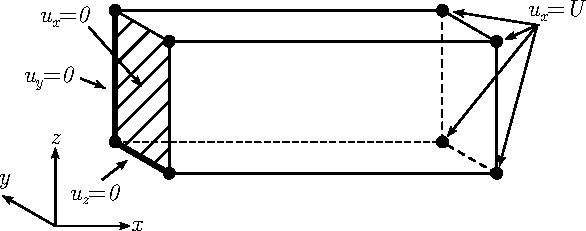
\includegraphics[width=0.8\linewidth]{tensileSetup.pdf}
    \caption[Displacement boundary conditions for dislocation plasticity modelling of single crystal micro-tensile tests.]{Displacement boundary conditions for dislocation plasticity modelling of single crystal micro-tensile tests.}
    \label{f:tensileSetup}
\end{figure}

In EasyDD, time is defined in units of shear modulus, which has SI units of $\left[\si{\kilo\gram\cdot\metre^{-1}\cdot\second^{-2}}\right]$. We know the displacement rate used in the experiments has units of $\left[\si{\metre\cdot\second^{-1}}\right]$. For a uniaxial loading scenario on a cuboid domain, obtaining the displacement rate, is fairly straight forward. We want a stress that when distributed along the loaded dimension, will give us the experimental one,
\begin{align}
    \dot{u}_\rvar{emp} \equiv \dfrac{\Delta l}{\Delta t} =
    \dot{u}_\rvar{sim} \equiv \dfrac{L}{\mu} \to
    \Delta t \equiv \dfrac{\Delta l \mu}{L} \therefore
    \dot{u}_\rvar{sim} = \dfrac{L}{\Delta t} = \dfrac{L^2}{\Delta l \mu}\,,
\end{align}
where $L$ is the dimension along the loaded axis, $\mu$ the material's shear modulus, $\Delta l$ the experimental displacement over a $\Delta t$ time interval. Since we use micron units, the displacement and shear modulus have been converted to them.

\subsection{Results and discussion}
\subsection{Conclusions}

\section{Tungsten cyclic loading and unloading cantilever}\label{s:tungstenCyclic}
\subsection{Introduction}
\subsection{Methodology}
\subsection{Results and discussion}
\subsection{Conclusions}

% 310